\chapter{Method}
\label{chap:method}
%Describe earlier approach:
%
%Rule based v(s,o) matching
%
%How this led to trying more generalizable approaches:
%
%Describe current process:
%
%dependency parsing gigacorpus to ldh, xdh, xdx formats;
%
%(gigacorpus info -- did I use full corpus or sample? check)
%
%same for PDT responses;
%
%dependency-based tf-idf for responses vs. gigacorpus;
%
%get sorted superset of XGS \& response terms and their tf-idf scores;
%
%get cosine of these vectors (``TC'' for tf-idf cosine; discuss how this compares to recent encoder based approaches (BERT), as this essentially is a primitive, more transparent encoder);
%
%rank responses by TC;
%
%get spearman of XGS \& TC based ranking vs ranking via the weighted feature annotations.
%
\section{Introduction}
In this chapter, I explain my system for rating and ranking responses automatically, where the goal is to approximate the benchmark rankings described in Chapter~\ref{chap:annotation}. 
The data-driven method used to analyze picture description task (PDT) responses throughout this dissertation represents an evolution from my own previous rule-based method. In this chapter, I briefly summarize this earlier study and the lessons learned there, then lay out the current approach.

In short, my first approach was heavily rule-based and relied on strict matching with a pre-established set of acceptable responses. This found moderate success, but lead to the current approach, which is data-driven and relies on more flexible methods of comparison. 

%In short, my earlier approach assessed each non-native speaker (NNS) response by extracting a \textit{verb(subject,object)} triple and looking for a match among triples from the native speaker (NS) responses. This involved dependency parsing the sentence then applying custom rules based on the labels, relationships and parts of speech in order to find each element of the triple. This process found moderate success, correctly assessing roughly half of NNS responses with a very small number of NS responses. Considerable weaknesses emerged, however; the rule based approach meant that it was limited in its ability to handle variation, and the use of simple triples was a hacky simplification of meaning. This lead me to the current approach, which uses a more robust representation of meaning and replaces the rule based matching with measures of semantic similarity. These changes make for a more generalizable approach.

%%%% BEGIN material from Qual Paper (BEA 2013) %%%%
\section{Previous approach: Rule-based semantic triple matching}
\label{sec:first-approaches}
%% I feel like this needs some kind of tldr up front...
This section summarizes relevant work first presented in \citet{king:dickinson:13} and \citet{king:dickinson:14}; please see those papers for deeper discussions.

Like the current research, my previous work focused on analyzing English non-native speaker (NNS) responses to a PDT by comparison with (native speaker) NS responses. I was initially unsure if such a task would be within reach for a single researcher using off-the-shelf tools, so this study sought to uncover challenges and determine whether variation in the form and content of responses could be manageable.

%Research in SLA often
%relies on the ability of task design to induce particular linguistic
%behavior \citep{skehan1998assessing}, and the PDT should induce
%interactive behavior.  Moreover, the use of the PDT as a reliable
%language research tool is well-established in areas of study ranging
%from SLA to Alzheimer's disease \citep{ellis2000task,
%  forbes2005detecting}.

%The NNSs were intermediate and upper-level adult English learners in
%an intensive English as a Second Language program at Indiana
%University. We rely on visual stimuli here for a number of
%reasons. Firstly, computer games tend to be highly visual, so
%collecting responses to visual prompts is in keeping with the nature
%of our desired ILT. Secondly, by using images, the information the
%response should contain is limited to the information contained in the
%image. Relatedly, particularly simple images should restrict elicited
%responses to a tight range of expected contents.

\subsection{Rule-based matching method}
\label{sec:rule-method}

My earlier method was inspired by research from areas such as sentiment analysis, topic modeling, and content assessment that used rule-based approaches to extract important elements from dependency-parsed text (citations XYZ)\lk{XYZ}. My idea was to extract a \textit{verb(subj,obj)} triple from each sentence. Each NNS triple could be compared against the list of NS triples for a match; a NNS response with a NS triple match would be ``correct,'' while a non-match would be ``incorrect.''
%This research is motivated by a desire to see intelligent computer-assisted language learning (ICALL) applications move toward natural communication in game-like visual contexts, so I determined that a picture description task (PDT) would produce a fitting dataset. Research in second language acquisition (SLA) often relies on the
%ability of task design to induce particular linguistic behavior
%\citep{skehan1998assessing}, and the PDT should induce context-focused
%communicative behavior. PDT data allows one to investigate
%pure interlanguage without the influence of verbal prompts and shows
%learner language being used to convey meaning and not just manipulate forms.

For these experiments, I chose or developed PDT images that present an event that I believed to be transitive in nature and likely to elicit responses with an unambiguous subject, verb and object.

\begin{figure}[htb!]
%[width=0.8\columnwidth]
\begin{center}
\begin{tabular}{|c|}
\hline
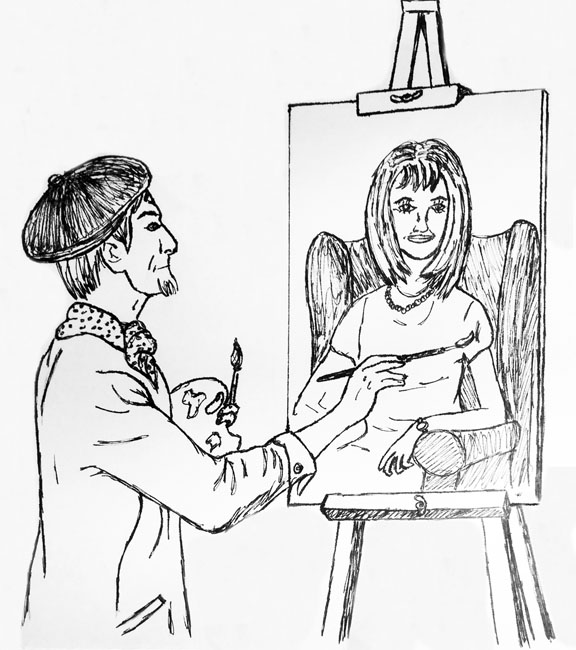
\includegraphics[width=0.55\columnwidth]{figures/exampleprompt.jpg}\\
\hline
\textbf{Response (L1)} \\
\hline
He is droning his wife pitcher. (Arabic)\\
\hline
The artist is drawing a pretty women. (Chinese) \\
\hline
The artist is painting a portrait of a lady. (English) \\
\hline
The painter is painting a woman's paint. (Spanish)\\
\hline
\end{tabular}
\end{center}
\caption{Example item and NNS responses from previous study.}
\label{fig:example-picture}
\end{figure}

The PDT consisted of 10 items (8 line drawings and 2 photographs) intended to elicit a single sentence each; an example is given in Figure~\ref{fig:example-picture}. Participants were asked to view the image and ``describe the action in either past or present tense.'' Responses were typed by the participants themselves in a computer lab with spell checking disabled.
I collected responses from 53 participants for a total of 530 sentences. There were 14 NSs (non-linguistics undergraduate and graduate students) and 39 NNSs (university students enrolled in English as a Second Language courses).

My process was to parse a NNS sentence into a dependency representation
%(section~\ref{sec:syntactic-form})
and then extract and lemmatize a semantic triple from this parse
%(section~\ref{sec:semantic-form})
to compare to a set of gold standard semantic triples similarly derived from the NS responses. As in my current research, I used the Stanford Parser for this task, trained on the Penn Treebank \citep{demarneffe:ea:06, klein:manning:03}.\footnote{\url{http://nlp.stanford.edu/software/lex-parser.shtml}} 

I manually categorized the 530 sentences in the dataset into 11 types plus one catch-all category, as shown in
Table~\ref{tab:sentence-type}. I established these types because each
one corresponds to a basic sentence structure and thus has consistent
syntactic features, leading to predictable patterns in the dependency
parses.


%\subsection{Obtaining a syntactic representation}
%\label{sec:syntactic-form}
%Because dependency parsing focuses on identifying dependency
%relations, rather than constituents or phrase structure, it clearly
%labels the subject, verb and object of a sentence, which can then map
%to a semantic form \citep{Kuebler.McDonald.Nivre-09}. In these experiments, I took a na\"ive approach in which subject, verb and
%object were considered sufficient for deciding whether or not a
%response accurately describes the visual prompt.

%
%Using the parser's options, I set the output to be Stanford typed
%dependencies, a set of labels for dependency relations. The Stanford
%parser has a variety of options for the specific
%ouput, e.g., how one wishes to treat prepositions
%\citep{defmarneffe:manning:12}.  I used only two non-default parser options ({\tt
%  CCPropagatedDependencies} and {\tt CCprocessed}\footnote{\url{http://nlp.stanford.edu/software/dependencies_manual.pdf}}) in order to:
%%
%1) omit prepositions and conjunctions from the sentence text and
%instead add the word to the dependency label between content words;
%and 2) propagate relations across conjunctions.  These decisions
%are important to consider for any semantically-informed processing of
%learner language.
%
%To see the impetus for removing prepositions, consider the learner
%example in Figure~\ref{fig:prep-dependency}, where the preposition \textit{with} is
%relatively unimportant to collecting the meaning.  Additionally,
%learners often omit, insert, or otherwise use the wrong preposition
%\citep{chodorow:et:al:07}.  The default parser would present a
%\texttt{prep} relation between \textit{played} and \textit{with},
%obscuring what the object is; with the options set as above, however,
%the dependency representation folds the preposition into the label
%(\texttt{prep\_with}), instead of keeping it in the parsed string, as
%shown in Figure~\ref{fig:prep-dependency}.
%
%\begin{figure}[htb!]
%\begin{center}
%    \begin{dependency}[arc edge,text only label,label style={above}]
%    \begin{deptext}[column sep=.5em]
%      \textit{vroot} \& The \&[1em] boy \&[1em] played \& with \& a \&[1em] ball \\
%    \end{deptext}
%    \depedge{4}{3}{nsubj}
%    \depedge[arc angle=90]{1}{4}{root}
%    \depedge{4}{7}{prep\_with}
%%    \depedge[arc angle=35,edge style={dotted}]{7}{6}{det}
%%    \depedge[edge style={dotted}]{3}{2}{det}
%    \depedge[arc angle=35]{7}{6}{det}
%    \depedge{3}{2}{det}
%  \end{dependency}
%\end{center}
%\caption{Dependency parse showing collapsed preposition dependencies.}
%\label{fig:prep-dependency}
%\end{figure}
%
%%\lk{it may be worthwhile to add the conll parse for this example so it's clear how these graphs come about}
%This is a lenient approach to prepositions, as prepositions
%are not without semantic meaning---e.g., \textit{the boy played in a
%  ball} means something quite different from the \textit{with} example.  However, this option makes it moderately easier to compare the meaning to an expected semantic form (e.g., \textit{play(boy,ball)}).
%
%As for propagating relations across conjunctions, this also simplifies the representation somewhat and makes it easier to connect verbs and their arguments, as needed for the semantic
%form used in comparisons. For a conjunction like \textit{cats and dogs}, for example, the default settings would produce \texttt{cc(cats, and)} and \texttt{conj(cats, dogs)}, but the chosen settings would collapse this into \texttt{conj\_and(cats, dogs)}, omitting the dependency that merely labels a conjunction relation between the first conjunct and the conjunction.

%Given the rule-based approach to matching \textit{verb(subject,object)} triples, many dependency relations are irrelevant for the next step of obtaining a semantic form.  For example, in this work I ignored determiner (\texttt{det}) relations between a noun and its determiner, allowing for variability in how a learner produces noun phrases. 

%\subsection{Obtaining a semantic representation}
%\label{sec:semantic-form}
%
%\subsubsection{Sentence types}

\begin{table*}[htb!]
\begin{center}
\begin{tabular}{|c|l|l|r|r|}
\hline
Type & Description & Example & NS & NNS \\
\hline
 A & Simple declarative transitive & The boy is kicking the ball. & 117 & 286 \\
 \hline
 B & Simple + preposition & The boy played with a ball. & 5 & 23 \\
 \hline
 C & Missing tensed verb & Girl driving bicycle. & 10 & 44 \\
 \hline
 D & Missing tensed verb + preposition & Boy playing with a ball. & 0 & 1 \\
 \hline
 E & Intransitive (No object) & A woman is cycling. & 2 & 21 \\
 \hline
 F1 & Passive & An apple is being cut. & 4 & 2 \\
 \hline
 F2 & Passive with agent & A bird is shot by a man. & 0 & 6 \\
 \hline
 Ax & Existential version of A or C & There is a boy kicking a ball. & 0 & 0 \\
 \hline
 Bx & Existential version of B  or D & There was a boy playing with a ball. & 0 & 0 \\
 \hline
 Ex & Existential version of E & There is a woman cycling. & 0 & 0 \\
 \hline
 F1x & Existential version of F1 & There is an apple being cut. & 0 & 1 \\
 \hline
 F2x & Existential version of F2 & There is a bird being shot by a man. & 0 & 0 \\
 \hline
 Z & All other forms & The man is trying to hunt a bird. & 2 & 6 \\
 \hline
\end{tabular}
\end{center}
\caption{Sentence type examples, with distributions of types for
  native speakers (NS) and non-native speakers (NNS)}
\label{tab:sentence-type}
\end{table*}

%\subsubsection{Rules for sentence types}

A sentence type indicates that the subject,
verb, and object can be found in a consistent place in the parse,
e.g., under a particular dependency label.
For example, for simple transitive sentences (type \textit{A} in Table~\ref{tab:sentence-type}),
the words labeled {\tt nsubj}, {\tt root}, and {\tt dobj} 
pinpoint the necessary information.
Thus, the patterns for extracting semantic information---in the form
of \textit{verb(subj,obj)} triples---reference particular Stanford
typed dependency labels, part-of-speech (POS) tags, and locations
relative to word indices (see Figure~\ref{fig:conll}).

\begin{figure}[htb!]
\begin{center}
\begin{tabular}{|C{4em}|C{5em}|C{4em}|C{4em}|C{4em}|}
\hline
\textbf{Index} & \textbf{Word} & \textbf{POS} & \textbf{Head} & \textbf{Label} \\
\hline
0 & \textit{root} & ROOT & 0 & root \\
\hline
1 & the & DET & 2 & det \\
\hline
2 & boy & NN & 4 & nsubj \\
\hline
3 & is & VBZ & 4 & aux \\
\hline
4 & kicking & VBG & 0 & root \\
\hline
5 & the & DT & 6 & det \\
\hline
6 & ball & NN & 4 & dobj \\
\hline
\hline
    \multicolumn{5}{|c|}{\begin{dependency}[arc edge,text only label,label style={above}]
    \begin{deptext}[column sep=.5em]
      ROOT \& DET \&[1em] NN \& VBZ \&[1em] VBG \& DET \&[1em] NN \\
      \textit{root} \& The \&[1em] boy \& is \&[1em] kicking \& the \&[1em] ball \\
    \end{deptext}
    \depedge[arc angle=90]{5}{3}{nsubj}
    \depedge{5}{4}{aux}
    \depedge[arc angle=92]{1}{5}{root}
    \depedge[arc angle=80]{5}{7}{dobj}
%    \depedge[arc angle=35,edge style={dotted}]{7}{6}{det}
%    \depedge[edge style={dotted}]{3}{2}{det}
    \depedge[arc angle=35]{7}{6}{det}
    \depedge{3}{2}{det}
  \end{dependency}} \\
\hline
\end{tabular}
\end{center}
%\caption{The dependency parse of an example NNS response in CoNLL\footnote{Standard dependency parse format established by the Conference on Computational Natural Language Learning (CoNLL).} format and the corresponding visual representation.}
\caption{The dependency parse of an example NNS response in a standard format (CoNLL) and the corresponding visual representation.}
\label{fig:conll}
\end{figure}

%More complicated sentences or those containing common learner errors
%(e.g., omission of the copula \textit{be}) required slightly more
%complicated extraction rules, but, since this work examined only transitive
%verbs, these still boiled down to identifying the
%sentence type and extracting the appropriate triple.
Determining the sentence type is accomplished by arranging a small set of binary decisions into a tree, as shown in Figure~\ref{fig:decision-tree}. This decision tree checks for the presence of various dependency labels. The extraction rules for the particular sentence type are then applied to obtain the semantic triple. Finally, for each NNS response, the resulting triple was checked against the gold standard list of NS triples. Ideally, each acceptable response should find a match, and unacceptable responses should not.

\begin{figure*}[htb!]
\begin{center}
\begin{tikzpicture}
\tikzset{level distance=3.5em}
\tikzset{edge from parent/.append style={->}}
\Tree
[.{\tt expl}?
  \edge node[auto=right,pos=.6,inner sep=1pt]{Y};
  [.{\tt auxpass}? 
  	\edge node[auto=right,pos=.6,inner sep=1pt]{Y};
  	[.{\tt agent}? 
		\edge node[auto=right,pos=.6,inner sep=1pt]{Y};
		[.F2x ]
		\edge node[auto=left,pos=.6,inner sep=1pt]{N};
		[.F1x ]
	]
	\edge node[auto=left,pos=.6,inner sep=1pt]{N};
	[.{\tt dobj}? 
		\edge node[auto=right,pos=.6,inner sep=1pt]{Y};
		[.Ax ]
		\edge node[auto=left,pos=.6,inner sep=1pt]{N};
		[.{\tt prep\_}$\ast$?
			\edge node[auto=right,pos=.6,inner sep=1pt]{Y};
			[.Bx ]
			\edge node[auto=left,pos=.6,inner sep=1pt]{N};
			[.Ex ]
		]
	]
  ]
  \edge node[auto=left,pos=.6,inner sep=1pt]{N};
  [.{\tt nsubjpass}? 
  	\edge node[auto=right,pos=.6,inner sep=1pt]{Y};
  	[.{\tt agent}? 
		\edge node[auto=right,pos=.6,inner sep=1pt]{Y};
		[.F2 ]
		\edge node[auto=left,pos=.6,inner sep=1pt]{N};
		[.F1 ]
	]
	\edge node[auto=left,pos=.6,inner sep=1pt]{N};
	[.{\tt dobj}? 
		\edge node[auto=right,pos=.6,inner sep=1pt]{Y};
		[.{\tt nsubj}?
			\edge node[auto=right,pos=.6,inner sep=1pt]{Y};
			[.A ]
			\edge node[auto=left,pos=.6,inner sep=1pt]{N};
			[.C ]
		]
		\edge node[auto=left,pos=.6,inner sep=1pt]{N};
		[.{\tt nsubj}?
			\edge node[auto=right,pos=.6,inner sep=1pt]{Y};
			[.{\tt prep\_}$\ast$?
			 	\edge node[auto=right,pos=.6,inner sep=1pt]{Y};
				[.B ]
				\edge node[auto=left,pos=.6,inner sep=1pt]{N};
				[.E ]
			]
			\edge node[auto=left,pos=.6,inner sep=1pt]{N};
			[.D ]
			]
		]
	]
  ]
]
\end{tikzpicture}
\end{center}
\caption{Decision tree for determining sentence type and extracting semantic triple}
\label{fig:decision-tree}
\end{figure*}

%To illustrate, consider the process for the example in Figure~\ref{fig:F2-dependency}.  The
%sentence is passed through the parser to obtain the dependency parse shown.
%The parsed sentence then moves to the
%decision tree shown in Figure~\ref{fig:decision-tree}.
%At the top of the tree, the sentence is checked for an {\tt expl}
%(expletive) label; having none, it moves rightward to the {\tt
%  nsubjpass} (noun subject, passive) node. Because a {\tt
%  nsubjpass} label is found, the sentence moves leftward to the {\tt agent}
%node. This label is also found, and because the sentence has reached a terminal node, it is labeled as a type F2 sentence.
%
%
%With the sentence now typed as F2, specific F2 extraction
%rules are applied. The logical subject is taken from under the {\tt agent} label,
%the verb from {\tt root}, and the logical object from {\tt nsubjpass},
%to obtain \textit{shot(man,bird)}, which can be lemmatized to
%\textit{shoot(man,bird)}. 
%%Very little effort goes into this process:
%%the parser is pre-built; the decision tree is small; and the
%%extraction rules are minimal.
%
%This much is possible with relatively little effort in part due to the constraints in the
%pictures.  For figure~\ref{fig:example-picture}, for example,
%\textit{the artist}, \textit{the man in the beret}, and \textit{the
%  man} are all acceptable subjects, whereas if there were multiple men
%in the picture, \textit{the man} would not be specific enough.
%%In future work, we expect to relax such constraints on image contents
%%by including rules to handle relative clauses, adjectives and other
%%modifiers in order to distinguish between references to similar
%%elements, e.g., 
%%\textit{a man shooting a bird} vs. \textit{a man reading the
%%  newspaper}.

\subsection{Rule-based matching results}
\label{sec:rule-results}

Evaluating this work required addressing two major questions.  First,
how accurately does this approach extract semantic information from potentially
innovative sentences?
%Due to the simple structures of the sentences (section~\ref{sec:sentence-distribution}), this simple system performs moderately well.
Secondly, how many semantic forms does one need in order to capture the variability in meaning in NNS sentences? I operationalized this second question by asking how well a given set of NS semantic forms models a gold standard.
% (section~\ref{sec:eval:coverage})?

An accurate extraction was defined as one in which the extraction rules chose the desired subject, verb, and object given the sentence at hand and without regard to the PDT image. Accuracy was 92.3\% for NNS responses and 92.9\% for NS responses. I attribute the high extraction scores to the constrained nature of the task and the relatively small range of sentence types it elicits. As seen in Table~\ref{tab:sentence-type}, only three sentence types account for more than 90\% of all responses. 

Assessing the coverage of NNS forms required first manually determining which extracted triples \textit{should} be matched given a hypothetical perfect gold standard set of triples. To separate the problem of coverage from extraction, I removed any incorrectly extracted triples from the NNS set and the NS gold standard.
 
I called an appropriate NNS triple found in the gold standard set a \textbf{true positive (TP)} (i.e., a correct match), and an appropriate NNS triple \textit{not found} in the gold standard set a \textbf{false negative (FN)} (i.e., an incorrect non-match), as shown in Table~\ref{tab:contingencies}. I used standard terminology here (TP, FN), but because this was an investigation of what \emph{should be} in the gold standard, these were considered
false negatives and not false positives.  To address the question of
how many (NS) sentences are needed to obtain good coverage, \textbf{coverage} was defined as recall: \textit{TP/(TP+FN)}. I reported 23.5\% coverage for unique triple
types and 51.0\% coverage for triple tokens.

\begin{table}[htb!]
\begin{center}
\begin{tabular}{|ll||l|l|}
  \hline
  & & \multicolumn{2}{c|}{NNS}\\
  & & $+$ & $-$ \\
  \hline
  \hline
  \multirow{2}{*}{NS} & Y & TP & FP \\
  \cline{2-4}
  & N & FN & TN\\
  \hline
\end{tabular}
\end{center}
\caption{Contingency table comparing presence of NS forms (Y/N) with
  correctness ($+$/$-$) of NNS forms}
\label{tab:contingencies}
\end{table}

I defined an inappropriate NNS triple (i.e., a content error)
\textit{not found} in the gold standard set as a \textbf{true negative
  (TN)} (i.e., a correct non-match). \textbf{Accuracy} based on this
gold standard---assuming perfect extraction---is defined as
\textit{(TP+TN)/(TP+TN+FN)}.\footnote{Accuracy is typically defined as (TP+TN)/(TP+TN+FN+FP), but false positives (FPs) are cases where an incorrect NNS response was in the gold standard; by removing errors from the NS responses, I prevented this scenario (i.e., FP=0).} I reported 46.4\% accuracy for types and 58.9\% accuracy for tokens.

The immediate lesson taken from this was: given a strict matching approach, NS data alone does not make a sufficient gold standard, in that many correct NNS answers are not counted as correct. I explored expanding the set of NS triples by separating individual subjects, verbs and objects from NS triples and recombining them into the various possible combinations. However, this lead to new problems as it generates a lot of nonsensical triples. Consider, for example, \textit{do(woman,shirt)}---an incorrect triple derived from the correct NS triples, \textit{wash(woman,shirt)} and \textit{do(woman,laundry)}. Instead, my current work has attempted to improve coverage by prompting NSs to give an initial PDT response, followed by a second alternative.

A related concern was that, even when only examining cases
where the meaning is literally correct, NNSs produced a wider range of
forms to describe the prompts than NSs. For example, for a picture
showing what NSs overwhelmingly described as a \textit{raking} action,
many NNSs referred to a man \textit{cleaning} an area. Literally,
this may be true, but it does not align with a NS based gold standard. 
This behavior was expected, given that learners are encouraged
to use words they know to compensate for gaps in their vocabularies
\citep{AgustinLlach2010}. This also parallels the observation in SLA research that while second language learners may attain native-like grammar, their ability to use
pragmatically native-like language is often much lower
\citep{BardoviDornyei1998}. \lk{Work a D Stringer citation in here?}
These findings highlighted the need for a more flexible approach.
%that considers how native-like a sentence is as well as how appropriate its meaning is.

Moreover, evaluating this strict matching approach required an annotator to decide whether a given response is correct or incorrect. Partial matching is not allowed; this is an inherent weakness of the approach, because while a complete triple gives some indication of the meaning of the sentence, any single element of the triple taken alone does not provide enough context to indicate meaning. This inflexibility means that using this approach would effectively require the manual curation of a robust gold standard set of acceptable responses, which is counter to my goal of producing an approach that can be expanded to new PDT items simply by crowdsourcing a gold standard from NSs.

%\begin{table}[htb!]
%\begin{center}
%\begin{tabular}{|c|c|}
%\hline
%Triple & Example sentence \\
%\hline
%\hline
%shoot(man, bird) & A man just shot a bird. \\
% \hline
%shoot(man, fowl) & The man shoots the fowl. \\
% \hline
%shoot(man, duck) & A man just shot a duck. \\
% \hline
%shoot(hunter, bird) & The hunter has shot a bird. \\
% \hline
%shoot(he, bird) & He shot the bird down! \\
% \hline
% \end{tabular}
%\end{center}
%\caption{The NS gold standard for Item 10.}
%\label{tab:item10GS}
%\end{table}

I followed up this work with a modification of this strict matching approach that included  language models and spell checking tools to attempt to identify and fix misspellings that lead to downstream problems \citep{king:dickinson:14}. I omit this discussion because it is not applicable to the current work; I now take a simpler approach --- respondents use spell checking during the task. This is because in most contexts where my system would be used, like a language tutoring application or game, spelling instruction is not the objective, and a built-in spell checker would likely be available. Moreover, omitting this step removes a layer of analysis---and importantly, a potential source of errors---and allows the research to focus more directly on meaning.

%%%% END material from Qual Paper (BEA 2013) %%%%


%%%% BEGIN material from BEA 2016 %%%%
\section{Recent work: Generalized, similarity-based approaches}

%%%% 2020/05/21. Resume here. %%%% 

In subsequent work \citep{king:dickinson:16}, I began looking for a ``sweet spot'' of
semantic analysis \citep[cf.][]{bailey:meurers:08} for image-based learner productions. I applied new methods to the same dataset, and the current dissertation research applies a refined version of these methods to the new dataset discussed in Chapters~\ref{chap:data} and~\ref{chap:annotation}.
In particular, using available NLP tools, I moved away from specific correct semantic representations and an exact definition of correctness, to more abstract representations
and more gradable notions of correctness (section~\ref{sec:ranking}). This obviates the need for a rule-based extraction of sentence elements, which must be customized for a limited range of expected sentence types. It also allows for graded scoring of results, meaning that a response is not outright rejected because only one element of a triple is not found. On the other hand, it means that the system does not provide a discrete ``acceptable'' or ``not acceptable'' decision, which means that downstream tasks like assessment, providing feedback or effecting game outcomes would require more careful consideration of what to do with the system output.

I should note, in this context, that I am discussing semantic
analysis given a gold standard set of NS sentences.  Image processing
tasks often rely on breaking images into semantic primitives
\citep[see, e.g.,][and references therein]{ortiz:wolff:lapata:15}, but
for NNS data, I want to ensure that I can account not just for
correct semantics (the \emph{what} of a picture), but natural
expressions of the semantics (the \emph{how} of expressing the
content).  In other words, the goal is to reason about meaning based on
specific linguistic forms.

A second issue regarding content analysis, beyond correctness, stems
from using an incomplete GS. The productive nature of language means that a sentence can be expressed in countless ways, and thus a GS can never really be ``complete''. Examining the degree of this variability both for NSs and NNSs is necessary to determine whether a crowd-sourced gold standard can account for a sizable portion of test responses. Analyzing variability can also help determine the most effective parameters for an NLP system for image based responses. Additionally, it can offer insights into theoretical research on variability in learner language (cf. \citet{ellis1987variability}, \citet{kanno1998consistency}).

%That is, different types of image content might require
%different mechanisms for processing.  Additionally, knowing how
%different pictures elicit different kinds of content can provide
%feedback on appropriate types of new data to collect.
%We approach this issue by clustering responses in various ways
%(section~\ref{sec:clustering}) and seeing how the clusters connect to
%system parameters.
%
%For both the experiments involving the accuracy of different system
%parameters (section~\ref{sec:ranking}) and the clustering of different
%responses (section~\ref{sec:clustering}), we present results within
%those sections that show the promise of moving to abstract representations, but in
%different ways for different kinds of data.
%
%We build directly from \citet{king:dickinson:13,king:dickinson:14},
%where the method to obtain a semantic form from a NNS production is:
%1) obtain a syntactic dependency representation from the off-the-shelf
%Stanford Parser \citep{demarneffe:ea:06, klein:manning:03}, and 2)
%obtain a semantic form from the parse, via a small set of hand-written
%rules.  It is this method we attempt to generalize
%(section~\ref{sec:ranking}).

%\section{Data Collection}
%\label{sec:data}
%
%Because our approach requires both NS and NNS responses and
%necessitates constraining both the form and content of responses, we
%previously assembled a small corpus of NS and NNS responses to a PDT
%\citep{king:dickinson:13}.  Research in SLA often relies on the
%ability of task design to induce particular linguistic behavior
%\citep{skehan1998assessing}, and the PDT should induce context-focused
%communicative behavior.  Moreover, the use of the PDT as a reliable
%language research tool is well-established in areas of study ranging
%from SLA to Alzheimer's disease \citep{ellis2000task,
%forbes2005detecting}.

%
%The PDT consists of 10 items (8 line drawings and 2 photographs\footnote{We have not observed substantial differences between responses for the drawings and the photographs.}) intended to elicit a single sentence
%each; an example is given in Figure~\ref{fig:example-picture}. Participants
%were asked to view the image and describe the action in past or present tense.
%The data consist of responses from 53 informants (14 NSs, 39 NNSs),
%for a total of 530 sentences, with the NNSs being intermediate and
%upper-level adult English learners in an intensive English as a Second
%Language program.  The distribution of first languages (L1s) is: 14
%English, 16 Arabic, 7 Chinese, 2 Japanese, 4 Korean, 1 Kurdish, 1
%Polish, 2 Portuguese, and 6 Spanish.
%
%Responses were typed by the participants themselves, with spell checking disabled in some cases.  Even among the NNSs that used spell checking, a number of spelling errors resulted in real words. To address this, we use a spelling correction tool to obtain candidate spellings for each word, prune the candidates using word lists from the NS responses, recombine candidate spellings into candidate sentences, and evaluate these with a trigram language model (LM) to select the most likely intended response \citep{king:dickinson:14}.
%
%Once the responses had been collected, the NNS responses were
%annotated for correctness, with respect to the content of the picture.
%The lead author marked spelling and meaning errors which prevent a
%complete mapping to correct information
%\citep[see][]{king:dickinson:13}.  On the one hand, minor misspellings
%are counted as incorrect (e.g., \textit{The artiest is drawing a
%\textbf{portret}}), while, on the other hand, the annotation does
%not require distinguishing between between spelling and meaning
%errors.  In the future, we plan on fine-tuning the annotation
%criteria.
\bigskip
START HERE 2021/01/15
\bigskip

\subsection{Generalizing the Methods}
\label{sec:ranking}

The previous work assumed that the assessment of NNS responses
involves determining whether a gold standard set contains the same
semantic triple that the NNS produced, i.e., whether a \textit{triple}
is \textit{covered} or \textit{non-covered}.  In such a situation the
gold standard need only be comprised of \textit{types} (not \textit{tokens}) of semantic triples. But the gold standard is comprised of the small set of NS responses---here, only 14---and is thus incomplete. This means that exact matching is going to miss many cases,
and indeed as discussed in Section~\ref{sec:rule-results}, coverage was only at 51\%. Even with a much larger sample of NS responses, a gold standard will always be incomplete. Additionally, relying on matching of triples limits the utility of the method to specific semantic requirements, namely transitive sentences.  By changing to ``bags of dependencies'' and tallying the counts of dependencies in the NS responses comprising the gold standard, I moved into a gradable, or ranking, approach to NNS responses.

My goal is to emphasize the degree to which a response conveys the same
meaning as the GS, necessitating an approach which can automatically
determine the importance of a piece of information in the GS.  In Section~\ref{sec:representation}, I detail how I represented the information
 and in Section~\ref{sec:scoring}, I discuss comparing NNS
information to GS information, which allowed me
to rank responses from least to most similar to the GS.\footnote{Although rankings often go from highest to lowest, I prioritize identifying problematic cases, so I rank accordingly.}
%I also discuss the handling of various other system parameters (section~\ref{sec:parameters}).

This work used the same 10 item PDT dataset described in section~\ref{sec:first-approaches}. Another example is shown in Figure~\ref{fig:example-picture2}.

\begin{figure}
\begin{center}
\begin{tabular}{|c|}
\hline
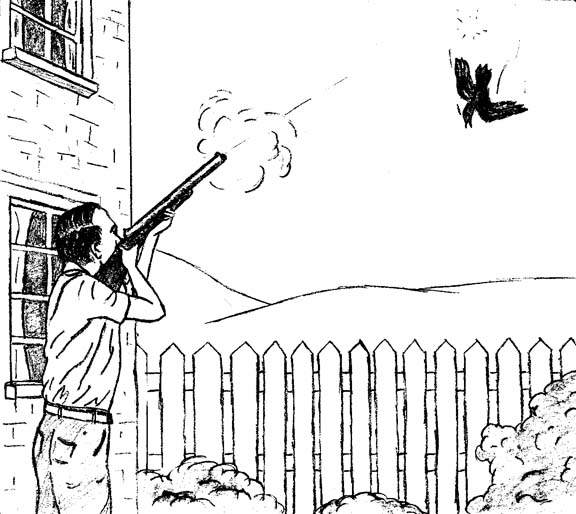
\includegraphics[width=0.7\columnwidth]{figures/exampleprompt2.jpg}\\
\hline
\textbf{Response (L1)} \\
\hline
The man killing the beard. (Arabic)\\
\hline
A man is shutting a bird. (Chinese) \\
\hline
A man is shooting a bird. (English) \\
\hline
The man shouted the bird. (Spanish)\\
\hline
\end{tabular}
\end{center}
\caption{Example item and responses}
\label{fig:example-picture2}
\end{figure}

\subsection{Representation}
\label{sec:representation}

To overcome the limitations of an incomplete GS, I represented each
response as a list of \textit{terms} taken from the dependency parse
\citep{demarneffe:ea:06}, the terms referring to
%being either 
individual dependencies (i.e., relations between words).
%or individual words. 
This eliminates the complications of extracting semantic triples from
dependency parses, which only handled a very restricted set of
sentence patterns and resulted in errors in 7--8\% of cases
\citep{king:dickinson:13}. Operating directly on individual
%words or
dependencies from the overall tree also means the system can allow for
``partial credit''; it distributes the matching over smaller,
overlapping pieces of information rather than a single, highly
specific triple.

Specifically, representations took one of five forms.  I first
tokenized and lemmatized a response to a list of dependencies that
represents the response.
The five term representations are then variations on dependencies. The
full form concatenates the label, head and dependent, as in
\texttt{subj\#boy\#kick}. I call this \textbf{ldh} (label, dependent,
head). The remaining four forms abstract over either the label, head
and/or dependent, as in \texttt{X\#boy\#kick}. I refer to these forms
as \textbf{xdh}, \textbf{lxh}, \textbf{ldx}, and \textbf{xdx}. I tested the system performance using each of these term representations separately.

The \param{xdx} model is on a par with treating the sentence as a ``bag
of words'' (or more accurately, a bag of lemmas), except that some function words not receiving parses (e.g., prepositions) are not included (see section~\ref{sec:syntactic-form}).

\subsection{Scoring Responses}
\label{sec:scoring}

Taking the term representations from the previous section, my next
step was to combine them in a way which ranks responses from least to
most appropriate.  I scored the responses with one of four approaches, each
using one of two methods to \textbf{weight} response terms combined
with one of two methods to \textbf{compare} the weighted NNS terms
with the GS.

For weighting, I used either a simple frequency measure
or one based on term frequency-inverse document frequency (\textbf{tf-idf})
\citep[][ch. 6]{manning-et-al:08}.  I used tf-idf as a measure of
a term's importance with the hope that it could reduce the impact
of semantically unimportant terms---e.g., determiners like
\textit{the}, frequent in the GS, but unimportant for evaluating the
semantic contents of NNS responses---and to upweight terms which may
be salient but infrequent, e.g., only used in a handful of GS
sentences. For example, for an item depicting a man shooting a bird
(see Table~\ref{tab:i10responses-avgprec} and Figure~\ref{fig:example-picture}), of 14 GS responses, 12
described the subject as \textit{man}, one as \textit{he} and one as
\textit{hunter}. Since \textit{hunter} is relatively infrequent in English, even
one instance in the GS should get upweighted via tf-idf, and indeed it
that was the effect. 
This is valuable, as numerous NNS responses used \textit{hunter}.

Calculating tf-idf relies on both \emph{term frequency} ($tf$) and
\emph{inverse document frequency} ($idf$).  Term frequency is simply
the raw count of a term, and for tf-idf of terms in the GS, I take
this as the frequency within the GS.  Inverse document frequency is
derived from some reference corpus, and it is based on the notion that
appearing in more documents makes a term less informative with respect
to distinguishing between documents.  The formula is in
(\ref{ex:tfidf}) for a term $t$, where $N$ is the number of documents
in the reference corpus, and $df_{t}$ is the number of documents
featuring the term ($idf_{t} = \log \frac{N}{df_{t}}$).  A term
appearing in fewer documents will thus obtain a higher $idf$ weight,
and this should readjust frequencies based on semantic importance.

\begin{exe}
\ex\label{ex:tfidf} $tfidf(t) = tf_{GS} \log \frac{N}{df_{t}}$
%, where $df_t = |\{d\in D, t \in d\}|$
\end{exe}

After this counting or weighting, the scores are then either
\textbf{averaged} to yield a response score, or NNS term
weights and GS term weights are treated as vectors and the response
score is the \textbf{cosine distance} between them.  This
yields:

%%former approach names: b = FA; m = IC (TC); c = FC; a = IA (TA)
\paragraph{Frequency Average (FA).} 
%This approach serves as our baseline. 
Within the GS, the frequency of each term is calculated. Each term in
the NNS response is then given a score equal to its frequency in the
GS; terms missing from the GS are scored zero. The response score is
the average of the term scores, with higher scores closer to the GS.

\paragraph{Tf-idf Average (TA).} This involves the exact same
averaging as with model FA, but now the terms in the GS are assigned
tf-idf weights before averaging.

\paragraph{Frequency Cosine (FC).} The frequency of each term is
calculated within the GS and (separately) within the NNS response. 
The term scores are then treated as vectors, and the response score is
the cosine distance between them, with lower scores being closer to
the GS.

\paragraph{Tf-idf Cosine (TC).} This involves the exact same
distance comparison as with model FC, but now the terms of both the GS
and NNS responses are assigned tf-idf weights before comparison.

The two cosine approaches are effectively primitive versions of sentence encoders like the currently popular BERT \citep{BertDevlin2018} and Universal Sentence Encoder \citep{UniversalSentenceEncoder}. Sentence encoders are a form of language model that learns mathematical representations of words by observing them in context, accounting for things like average distance from a given word type to another given word type. Sentence encodings are thus vectors representing these word values for a full sentence. These approaches result in very high dimensional spaces---imagine a sentence representation that consists of a vector for each word in the sentence, where each vector is a list of average distances from that word type to \textit{every other word type in the language}. Thus sentence encoders typically rely on methods of dimensionality reduction to compress these representations into vectors of manageable length.
I say my cosine approaches constitute ``primitive'' encoders because they omit this step. In the case of my PDT constrained corpus, the number of word types (and in turn dependency types) observed for a given item remains small enough that the raw vectors representing dependencies' tf-idf scores can still be processed easily with a laptop computer. Not only does this simplify the process, it means that the process remains transparent. There are no opaque machine learning processes that derive compressed representations, and each sentence vector could be examined value by value, where each number represents a real dependency. This is important because it leaves the door open for meaningful feedback on each response. For example, one could identify the most salient dependencies in the GS of a given item and somehow present those to a user who gives a low scoring response in order to suggest a more appropriate response. That is to say, a full encoder could determine how similar a response is to a GS, but it could not tell us \textit{why} it made its determination.

\subsection{System Parameters}
\label{sec:parameters}

In addition to the four approaches, the five term representations and
two sets of parameters, listed below, were varied, resulting in a total of
60 settings for processing responses (see also
Table~\ref{tab:dist-ranked-parameters}). 

\paragraph{Term form.} As discussed in
section~\ref{sec:representation}, the terms can take one of five
representations: \param{ldh}, \param{xdh}, \param{lxh}, \param{ldx},
or \param{xdx}.

\paragraph{Scoring approach.} As discussed in
section~\ref{sec:scoring}, the NNS responses can be
compared with the GS via models \param{FA}, \param{TA}, \param{FC}, or \param{TC}.

\paragraph{Reference corpus.} The reference corpus for deriving tf-idf
scores can be either the Brown Corpus \citep{kucera:francis:67} or the
Wall Street Journal (WSJ) Corpus \citep{marcus-et-al:93}. These are
abbreviated as \param{B} and \param{W} in the results
below; \param{na} indicates the lack of a reference corpus, as this is
only relevant to approaches \param{TA} and
\param{TC}. The corpora are divided into as many documents as
originally distributed (\param{W}: 1640, \param{B}: 499). The WSJ is
larger, but Brown has the benefit of containing more balance in its
genres (vs. newstext only). Considering the narrative nature of PDT
responses, a reference corpus of narrative texts would be ideal, but
I chose manually parsed reference corpora as they are more reliable
than automatically parsed data.

\paragraph{NNS source.} Each response has an original version
(\param{NNSO}) and the output of a language model spelling corrector
(\param{NNSLM}). (The current dissertation relies on a corpus for which participants used spell checking at the time of the task, so this offline spelling correction is no longer applicable. In short, it used a spelling tool to find candidate spellings for each word in a NNS sentence, pruned the lists of candidate words by comparing against words in NS responses, formed new candidate sentences by combining candidate words, and finally chose the most likely sentence by rating each candidate with a trigram word model. I omit the exact details here for brevity, but more can be found in \cite{king:dickinson:14}).

\subsection{Results}

\subsubsection{Evaluation metrics}
\label{sec:metrics}

I ran 60 response experiments, each with different system settings
(section~\ref{sec:parameters}). Within each experiment, I ranked the 39
scored NNS responses from least to most similar to the GS.

For assessing these settings themselves, I relied on the past annotation,
which counted unacceptable responses as errors (see
section~\ref{sec:eval:extraction}).  As the
lowest rank indicates the greatest distance from the GS, a good system
setting should ideally position the unacceptable responses among those
with the lowest rankings. Thus, I assigned each error-containing
response a score equal to its rank, or, if necessary, the average rank
of responses sharing the same score.

In Table~\ref{tab:i10responses-avgprec}, an excerpt of sentence
responses is shown for one item, ranked from lowest to highest.  To
take one example, the third-ranked sentence, \textit{the man is hurting duck}, has a score of 0.996, and it is annotated as an error (1 in
the \textit{E} column).  Thus, the evaluation metric adds a score of 3
to the overall sum.  The sentence ranked 18, by contrast, is not an
error, and so nothing is added.  In the case of the top rank, two
responses with errors are tied, covering rank 1 and 2, so each adds a score of 1.5.

\begin{table}[htb!]
\begin{center}
\setlength{\tabcolsep}{0.3em}
\begin{tabular}{|r|c|l|r|r|}
\hline
\textit{R} & \textit{S} & Sentence & \textit{E} & \textit{V}\\
\hline
\hline
\multirow{2}{*}{1} & 1.000 & she is hurting. & 1 & 1.5 \\
& 1.000 & man mull bird & 1 & 1.5 \\
\hline
3 & 0.996 & the man is hurting duck. & 1 & 3.0 \\
4 & 0.990 & he is hurting the bird. & 1 & 3.0 \\
\hline
11 & 0.865 & the man is trying to hurt a bird & 1 & 11.0 \\
12 & 0.856 & a man hunted a bird. & 0 & 0.0 \\
\hline
17 & 0.775 & the bird not shot dead.  & 1 & 17.0 \\
18 & 0.706 & he shot at the bird & 0 & 0.0 \\
19 & 0.669 & a bird is shot by a un & 1 & 19.0 \\
20 & 0.646 & the old man shooting the birds & 0 & 0.0 \\
\hline
37 & 0.086 & the old man shot a bird. & 0 & 0.0 \\
38 & 0.084 & a old man shot a bird. & 0 & 0.0 \\
39 & 0.058 & a man shot a bird & 0 & 0.0 \\
\hline
\hline
\multicolumn{3}{|c|}{Total (Raw)} & 17 & 169 \\
\hline
\multicolumn{3}{|c|}{Average Precision} & \multicolumn{2}{c|}{0.75084} \\
\hline
\end{tabular}
\caption{Rankings for Item 10 from the best system setting (tf-idf cosine scoring, Brown Corpus for tf-idf reference, the language model spelling corrected NNS sentence, and the full label, dependent and head representation; TC\_B\_NNSLM\_ldh) based on average precision scores. \textit{R}: rank; \textit{S}: sentence score; \textit{E}: error; \textit{V}: rank value. Note that not all responses are shown. }
\label{tab:i10responses-avgprec}
\end{center}
\end{table}

The sum of these scores is taken as the \textbf{Raw} metric for that
experimental setting. In many cases, one version of a response
(\param{NNSO} or \param{NNSLM}) contains an error, but the other
version does not. Thus, for example, an \param{NNSO} experiment may
result in a higher error count than the \param{NNSLM} equivalent, and
in turn a higher Raw score.
In this sense, Raw scores emphasize error reduction and incorporate
item difficulty.

However, it is possible that the \param{NNSO} experiment, even with
its higher error count and Raw score, does a better job ranking the
responses in a way that separates good and erroneous ones. To account
for this, I also used \textbf{(mean) average precision ((M)AP)}
\citep[][ch. 8]{manning-et-al:08}, which emphasizes discriminatory
power.

For average precision (AP), one calculates the precision of error
detection at every point in the ranking, lowest to highest.  In
Table~\ref{tab:i10responses-avgprec}, for example, the precision for
the first cut-off (1.000) is 1.0, as two responses have been
identified, and both are errors ($\frac{2}{2}$). At the 11th- and
12-ranked response, precision is 1.0 ($\frac{11}{11}$) and 0.917
(=$\frac{11}{12}$), respectively, precision dropping when the item is
not an error.
AP averages over the precisions for all $m$ responses ($m=39$ for our
NNS data), as shown in (\ref{ex:ap}), with each response notated as
$R_k$.  Averaging over all 10 items results in the Mean AP (MAP).

\begin{exe}
\ex\label{ex:ap} $AP(item) = \frac{1}{m} \sum\limits_{k=1}^m
Precision(R_k)$
\end{exe}

As mentioned, the Raw metric emphasizes error reduction, as it
reflects not just performance on identifying errors, but also the
effect of the overall number of errors.
%In this way, it may be useful
%for predicting future system performance, an issue we explore in the
%evaluation of clustering items (section~\ref{sec:clusteringresults}).
MAP, on the other hand, emphasizes finding the optimal separation
between errors and non-errors and is thus more of the focus in the
evaluation of the best system parameters next.

\subsubsection{Best system parameters} 

To start the search for the best system parameters, it may help to
continue with the example in
Table~\ref{tab:i10responses-avgprec}. The best setting, as determined by the
MAP metric, uses the tf-idf cosine (\param{TC}) approach with the Brown Corpus (\param{B}),
the spelling corrected response (\param{NNSLM}), and the full form of
the dependencies (\param{ldh}). It ranks highest because errors are
well separated from non-errors; the highest ranked of 17 total errors
is at rank 19.  Digging a bit deeper, one can see in this example how
the verb \textit{shoot} is common in all the highest-ranked cases shown
(\#37--39), but absent from all the lowest, showing both the effect of
the GS (as all NSs used \textit{shoot} to describe the action) and the
potential importance of even simple representations like lemmas.  In
this case, the \param{ldh} representation is best, likely because the
word \textit{shoot} is not only important by itself, but also in terms
of which words it relates to, and how it relates (e.g.,
\texttt{dobj\#bird\#shoot}).

\begin{table*}
\begin{center}
\begin{tabular}{|l|r||l|r||l|r||l|r|}
\hline
\multicolumn{2}{|c||}{Approach} & \multicolumn{2}{|c||}{Term Form} & \multicolumn{2}{|c||}{Ref. Corpus (TA/TC)} & \multicolumn{2}{|c|}{NNS Source} \\
\hline
\hline
0.51577 & TC & xdh & 0.51810 & Brown & 0.51534 & NNSLM & 0.51937 \\
\hline
0.50780 & FC & ldh & 0.51677 & WSJ & 0.50798 & NNSO & 0.49699 \\
\hline
0.50755 & TA & lxh & 0.51350 & & & & \\
\hline
0.49464 & FA & xdx & 0.49901 & & & & \\
\hline
& 	& ldx & 0.49352 &  &  &  & \\
\hline
\end{tabular}
\caption{Approaches and parameters ranked by mean average precision for all 10 PDT items.}
\label{tab:dist-ranked-parameters}
\end{center}
\end{table*}

Table~\ref{tab:all-dist-ranked-settings} shows the five best and five
worst system settings averaged across all 10 PDT items, as ranked by
MAP. Among the trends that pop out is a favoritism
towards \param{NNSLM} models (i.e., spelling correction). This is due
to the fact that higher numbers of errors inflate the MAP scores, and
somewhat counterintuitively, the spelling correction module introduces
more errors than it corrects, meaning there are more errors present
overall in the \param{NNSLM} responses than in the \param{NNSO}
responses.\footnote{Note that among the remaining parameter classes,
variation does not effect the number of errors.}

Another feature among the best settings is the inclusion of heads in the dependency representations. In fact, the top 17 ranked settings all include heads (\param{lxh}, \param{xdh}, \param{ldh}); \param{xdx} first enters the rankings at 18, and \param{xdx} and \param{ldx} are common among the worst performers. This is likely due to the salience of the verbs in these transitive sentences; they constitute the heads of the subjects and objects, in relatively short sentences with few dependencies.
Furthermore, the tf-idf weighted models dominate the rankings, especially \param{TC}. It is also clear that for my data tf-idf works best with the Brown Corpus (\param{B}).

\begin{table}[htb!]
\begin{center}
\begin{tabular}{|r|l|c|}
\hline
Rank & MAP & Settings \\
\hline
\hline
1 & 0.5534 & TC\_B\_NNSLM\_lxh \\
\hline
2 & 0.5445 & TA\_B\_NNSLM\_lxh \\
\hline
3 & 0.5435 & TC\_W\_NNSLM\_lxh \\
\hline
4 & 0.5422 & TC\_B\_NNSLM\_xdh \\
\hline
5 & 0.5368 & TC\_B\_NNSLM\_ldh \\
\hline
\hline
56 & 0.4816 & TA\_B\_NNSO\_xdx \\
\hline
57 & 0.4796 & FA\_na\_NNSLM\_ldx \\
\hline
58 & 0.4769 & FC\_na\_NNSO\_lxh \\
\hline
59 & 0.4721 & TA\_W\_NNSO\_xdx \\
\hline
60 & 0.4530 & FA\_na\_NNSO\_lxh \\
\hline
\end{tabular}
\caption{Based on Mean Average Precision, the five best and five worst settings across all 10 PDT items.}
\label{tab:all-dist-ranked-settings}
\end{center}
\end{table}

I also summarize the rankings for the individual parameter classes,
presented in Table~\ref{tab:dist-ranked-parameters}, confirming the
trends in Table~\ref{tab:all-dist-ranked-settings}. For a given
parameter, e.g., \param{ldh}, I averaged the experiment scores from
all settings including \param{ldh} across all 10 items. Notably, \param{TC} outperforms the other models, with \param{FC} and \param{TA} close behind (and nearly tied). Performance falls for the simplest model, \param{FA}, which was in fact intended as a baseline. With \param{TC}$>$\param{FC} and \param{TA}$>$\param{FA}, tf-idf weighting seems preferable to basic frequencies.

Again, the importance of including heads in dependencies is apparent here; the three dependency representations containing heads constitute the top three, with a sizable drop in performance for the remaining two forms (\param{xdx} and \param{ldx}). Moreover, given the content and narrative style of the PDT responses, it is unsurprising that the Brown Corpus serves as a better reference corpus than the WSJ Corpus for tf-idf. Finally, the \param{NNSLM} source significantly outperforms the \param{NNSO} source.

Despite the strength of these overall trends, variability
does exist among the best settings for different items, a point obscured
in the averages.  In Tables~\ref{tab:i01-dist-ranked-settings} and
\ref{tab:i05-dist-ranked-settings}, I present the best and worst
ranked settings for two of the least similar items, 1 and 5.
Their dissimilarity can be seen at a glance, simply from the range of
the AP scores (0.05--0.31 for item 1 vs. 0.52--0.81 for item 5), which
in itself reflects a differing number of erroneous responses (2 [\param{NNSO}]
or 6 [\param{NNSLM}] for item 1 vs. 23 or 24 for item 5).

For item 1, a drawing of a boy kicking a ball, there is considerable
variability in the best scoring approach just within the top five settings:
all four approaches (TA, TC, FA, FC) are in the top five.  Contrary to the overall
trends, I also found the \param{ldx} form---without any head
information---in the two best settings.  Note also that, even though
tf-idf weighting (\param{TA}/\param{TC}) is usually among the best settings, it is
occurs among the worst settings, too.

For item 5 in Table~\ref{tab:i05-dist-ranked-settings}, a drawing of a
man raking leaves, the most noticeable difference is that
of \param{xdx} being among three of the top five settings.
I believe that part of the reason for
the higher performance of \param{xdx} (cf. lemmas), is that for this
item, all the NSs use the verb \textit{rake}, while none of the NNSs use this word.  For item 1 (the boy kicking a ball), there is lexical variation
for both NSs and NNSs.

\begin{table}[htb!]
\begin{center}
\begin{tabular}{|r|c|c|}
\hline
Rank & AP & Settings \\
\hline
\hline
1 & 0.30997 & TC\_B\_NNSLM\_ldx \\
\hline
2 & 0.30466 & TA\_B\_NNSLM\_ldx \\
\hline
3 & 0.30015 & TA\_B\_NNSLM\_xdh \\
\hline
4 & 0.29704 & FC\_na\_NNSLM\_xdh \\
\hline
5 & 0.29650 & FA\_na\_NNSLM\_ldh \\
\hline
\hline
56 & 0.06474 & TC\_B\_NNSO\_ldx \\
\hline
57 & 0.06174 & TC\_W\_NNSO\_ldx \\
\hline
58 & 0.06102 & TA\_W\_NNSO\_lxh \\
\hline
59 & 0.05603 & TA\_W\_NNSO\_xdx \\
\hline
60 & 0.05094 & TA\_W\_NNSO\_ldx \\
\hline
\end{tabular}
\caption{Based on Average Precision, the five best and five worst settings for item 1.}
\label{tab:i01-dist-ranked-settings}
\end{center}
\end{table}

\begin{table}[htb!]
\begin{center}
\begin{tabular}{|r|c|c|}
\hline
Rank & AP & Settings \\
\hline
\hline
1 & 0.80965 & FA\_na\_NNSLM\_xdx \\
\hline
2 & 0.80720 & TA\_B\_NNSLM\_lxh \\
\hline
3 & 0.80473 & TC\_B\_NNSLM\_lxh \\
\hline
4 & 0.79438 & TC\_B\_NNSLM\_xdx \\
\hline
5 & 0.78108 & TC\_W\_NNSLM\_xdx \\
\hline
\hline 
56 & 0.56495 & FC\_na\_NNSO\_xdh \\
\hline
57 & 0.56414 & TC\_B\_NNSO\_lxh \\
\hline
58 & 0.55890 & TC\_W\_NNSO\_lxh \\
\hline
59 & 0.54506 & FC\_na\_NNSO\_lxh \\
\hline
60 & 0.52013 & FA\_na\_NNSO\_lxh \\
\hline
\end{tabular}
\caption{Based on Average Precision, the five best and five worst settings for item 5.}
%%LK: fixed 4/6 pm.
\label{tab:i05-dist-ranked-settings}
\end{center}
\end{table}

These types of differences---for these items and others---lead me to explore the clustering of item patterns, in order to
leverage these differences and automatically choose the optimal
settings for new items; we turn to this next.

%\section{Clustering}
%\label{sec:clustering}
%
%Given the variability of NS and NNS responses, and the possible
%correlation with different system parameters, we have begun exploring
%connections by clustering the different items.  The clustering uses,
%for one set, \emph{response features}, i.e., features observable from
%the responses, and, separately, \emph{performance features}, i.e., the
%performance of different system settings on the responses.
%
%Although the work is very exploratory, our goal is to get a handle on
%learner variability for different items and explore correlations
%between response and performance clusters.
%
%\subsection{Response Clustering}
%
%We cluster the 10 PDT items using simple features taken from the
%responses themselves. Specifically, we use various combinations of
%type counts, token counts, and type-to-token ratios for each term form
%(\param{ldh}, \param{xdh}, \param{lxh}, \param{ldx}, \param{xdx}),
%taken from each response source (GS, \param{NNSO}, \param{NNSLM}).
%
%\subsection{Performance Clustering}
%
%From the system output, we cluster items using per-item Raw 
%scores for various settings. That is, for each of the 10 items, we
%calculate an average error score for each approach
%(\param{FA}, \param{TA}, \param{FC}, \param{TC}), each term form
%(\param{ldh}, \param{xdh}, \param{lxh}, \param{ldx}, \param{xdx}),
%each reference corpus (\param{B}, \param{W}), and each
%response source (\param{NNSO}, \param{NNSLM}). 
%As mentioned in section~\ref{sec:metrics}, Raw scores should account for the number of
%errors produced by NNSs for each item, which should 
%correlate with future system performance.
%
%\subsection{Results}
%\label{sec:clusteringresults}
%
%Although there is noise in some experiments, some patterns do seem to
%emerge in many of the clusterings; we present some of the most common
%patterns here.
%
%Figure~\ref{fig:response-clusters} shows a clustering based on
%response features that shares some characteristics with
%Figure~\ref{fig:parameter-clusters}, a clustering based on performance
%features. (Note that clustering heights are not to scale.)  In both
%examples, items 5 and 9 form a cluster attaching to the root. These
%are described in the GS as \textit{A man is raking leaves} and
%\textit{Two boys are rowing a boat}. These were also the two most
%difficult items for NNSs. While other items involved common verbs like
%\textit{kick}, \textit{paint} and \textit{cut}, the actions depicted
%in these items were more specific and required words outside the
%vocabulary of many participants. For example, while all 14 NSs used
%either \textit{row} or \textit{paddle}, only five of 39 NNSs used
%these verbs; the rest used verbs like \textit{boat}, \textit{sail},
%\textit{sit}, \textit{play} or \textit{ride}.
%
%\begin{figure}
%\begin{center}
%\begin{tikzpicture}[sloped]
%\node (5) at (-7.5,0) {5};
%\node (9) at (-6.9,0) {9};
%\node (1) at (-6.2,0) {1};
%\node (4) at (-5.5,0) {4};
%\node (6) at (-4.7,0) {6};
%\node (2) at (-4.0,0) {2};
%\node (8) at (-3.2,0) {8};
%\node (10) at (-2.6,0) {10};
%\node (3) at (-1.8,0) {3};
%\node (7) at (-1.1,0) {7};
%\node (59) at (-7.2,0.7) {};
%\node (14) at (-5.9,0.7) {};
%\node (28) at (-3.5,0.7) {};
%\node (37) at (-1.5,0.7) {};
%\node (1037) at (-2.3,1) {};
%\node (281037) at (-2.9,1.3) {};
%\node (6281037) at (-3.6,1.7) {};
%\node (146281037) at (-4.9,2.1) {};
%\node (59146281037) at (-6.4,2.5) {};
%\draw  (5)  |- (59.center);
%\draw  (9)  |- (59.center);
%\draw  (1)  |- (14.center);
%\draw  (4)  |- (14.center);
%\draw  (2)  |- (28.center);
%\draw  (8)  |- (28.center);
%\draw  (3)  |- (37.center);
%\draw  (7)  |- (37.center);
%\draw (10) |- (1037.center);
%\draw (37) |- (1037.center);
%\draw (1037) |- (281037.center);
%\draw (28) |- (281037.center);
%\draw (6) |- (6281037.center);
%\draw (281037) |- (6281037.center);
%\draw (14) |- (146281037.center);
%\draw (6281037) |- (146281037.center);
%\draw (59) |- (59146281037.center);
%\draw (146281037) |- (59146281037.center);
%\end{tikzpicture}
%\end{center}
%\caption{PDT items clustered by type and token counts of all NS, NNSO and NNSLM responses.} 
%%%duh?%%(Heights not to scale.)}
%\label{fig:response-clusters}
%\end{figure}
%
%\begin{figure}
%\begin{center}
%\begin{tikzpicture}[sloped]
%\node (5) at (-7.5,0) {5};
%\node (9) at (-6.9,0) {9};
%\node (3) at (-6.2,0) {8};
%\node (8) at (-5.5,0) {3};
%\node (2) at (-4.7,0) {2};
%\node (10) at (-4.0,0) {10};
%\node (1) at (-3.2,0) {1};
%\node (4) at (-2.6,0) {4};
%\node (6) at (-1.8,0) {6};
%\node (7) at (-1.1,0) {7};
%\node (59) at (-7.2,.8) {};
%\node (210) at (-4.3,.7) {};
%\node (14) at (-2.9,.7) {};
%\node (67) at (-1.5,.7) {};
%\node (8210) at (-4.9,1.0) {};
%\node (38210) at (-5.7,1.3) {};
%\node (1467) at (-2.2,1.4) {};
%\node (382101467) at (-4,2) {};
%\node (all) at (-5,2.5) {};
%\draw  (5) |- (59.center);
%\draw  (9) |- (59.center);
%\draw  (2) |- (210.center);
%\draw  (10) |- (210.center);
%\draw  (1) |- (14.center);
%\draw  (4) |- (14.center);
%\draw  (6) |- (67.center);
%\draw  (7) |- (67.center);
%\draw  (8) |- (8210.center);
%\draw  (210) |- (8210.center);
%\draw  (8210) |- (38210.center);
%\draw  (3) |- (38210.center);
%\draw  (14) |- (1467.center);
%\draw  (67) |- (1467.center);
%\draw  (38210) |- (382101467.center);
%\draw  (1467)  |- (382101467.center);
%\draw  (59)  |- (all.center);
%\draw  (382101467)  |- (all.center);
%\end{tikzpicture}
%\end{center}
%\caption{PDT items clustered by parameter performance.} 
%%%duh?%%(Heights not to scale.)}
%\label{fig:parameter-clusters}
%\end{figure}
%
%Items 1 and 4 also appear as a cluster in both cases. In GS examples,
%these are described as \textit{The boy is kicking a ball} and
%\textit{A man is reading a newspaper}. The images portray actions that
%language learners often learn in beginner courses, and in fact, these
%were the easiest items for NNSs. The simple actions and objects mean
%that both token counts and type counts are relatively low. \md{Just to make sure: are these still the right parameters that perform highly?}\lk{I changed it slightly; these are best, but the trend isn't very strong via MAP. the trends are different via Raw, (and stronger, hence the cluster!) but I don't think we want to go into that, given that we present the MAP for item 1 in Table 4} With regard
%to feature performance, for both items the same parameters perform
%highly (\param{TC}/\param{TA}, \param{ldx}/\param{ldh}/\param{xdh}), suggesting that a future item
%which clusters with these two would benefit from the same processing.
%
%\section{Summary and Outlook}
%
%We have investigated ways to reason about learner meaning in cases
%where the set of correct meanings is incomplete, namely in the
%case of picture description tasks (PDTs).  Specifically, we have
%explored different models of representing and scoring NNS responses to
%a picture---different linguistic representations, term weighting
%schemes, reference corpora, and use of spelling correction---in order
%to automatically determine the relevant parts of an image from a set
%of NS responses.  In more exploratory work, we have also examined the
%variability in both NS and NNS responses, and how different system
%parameters correlate with the variability.  
%
%Already, the results are providing insight for future system
%development, data collection, and investigations into learner
%language. 
%A big next step of the work is to collect more data, and
%examining the variability in the NS/NNS data has provided feedback on
%the types of new data to gather, to better ensure a wide range of
%behavior from NNSs.  Getting a range of items, with different sentence
%types and variability in responses, will help us properly find our
%envisioned sweet spot of semantic analysis.  In that vein, we plan on
%exploring more parameters (e.g., semantic role information) and
%holding out data to better gauge the impact of clustering a new item
%with the existing items and selecting the processing parameters on
%that basis.

%%%% END material from BEA 2016 %%%%

\section{Current method}

The current method relies on a much larger corpus with more detailed annotation. As discussed in Chapter 4, the annotations do not encode for errors, as before, but instead give a binary score for five different features. This means the evaluation cannot take the form of MAP, but must instead compare response rankings, i.e., how well does the system rank responses in comparison to an ideal ranking based on manual annotations? Spearman rank correlation is used to provide these scores.

Because the annotations and evaluation are much different in the current work, it does not exactly follow that findings from the previous work will hold true. However, I believe that the previous work has highlighted some of the system parameters that are most likely to perform well, and I choose to experiment among the top contenders. For example, all of the current experiments rely on the tf-idf cosine (TC) approach, as this consistently outperformed the others. The frequency average (FA) approach is used \lk{Is it?} as a baseline where appropriate, as this presents a very simplistic distributional approach as opposed to the more linguistically sophisticated TC. The large increase in the size of the datasets also means that running an exhaustive search for the best parameters among all combinations is not reasonable; as discussed, the previous work used 60 different system settings in total. For that reason, I have chosen to focus on experiments that optimize for each parameter individually, then combine the best parameter settings for use on held out data to ensure they perform optimally. These experiments and their results are discussed in Chapter 6.

%TODO:
%This section should briefly summarize the takeaways from the chapter and explain which of the settings described here are used in the current experiments.
%Note that the current data is not annotated for errors, which means the current experiments rely on Spearman rank correlation scores, not MAP scores. This means I can't assume that the best settings found in 2016 will apply, but I should argue that the 2016 results do show some ability to discriminate as desired. and after all --- errors don't appear in the GS, and thus for our purposes they aren't native-like, and TC especially does seem to perform well here. Generally, the top settings seem fairly unsurprising and intuitive.
%This leads directly into the next chapter (Experiments), which contains a section for each experiment, which is basically varying a given parameter (ldh, xdh, xdx), and the results for each experiment.
%
%Question:
%Do I need some kind of baseline to compare to? Perhaps Frequency Average (FA)?